\documentclass[../../main/thesis_msc.tex]{subfiles}



\begin{document}

	%\chapter{\large Type-Ia Supernovae from non-accreting progenitors}
	\chapter{Results}
	
	
	In this chapter we present the results blah blah
	
	\newpage
	
	\null\newpage
	
	
	\section{Type-Ia Supernovae from non-accreting progenitors}\label{sec:results1}
	
	
		\vspace{3cm}
		
		 In this section, we present a novel progenitor channel for Supernovae-Ia along with a first-order approximation concerning the formation frequency of the corresponding progenitor systems, energetics of the explosion, and nucleosynthetic signature.
		
		\vspace{15cm}
		\noindent \textbf{Disclaimer}: What follows is an early draft version of the manuscript submitted for publication to \textit{ApJ Letters}. Differences may appear when compared with the published version. Hence, for citing this paper please refer to the journals.
		
		\newpage
	
		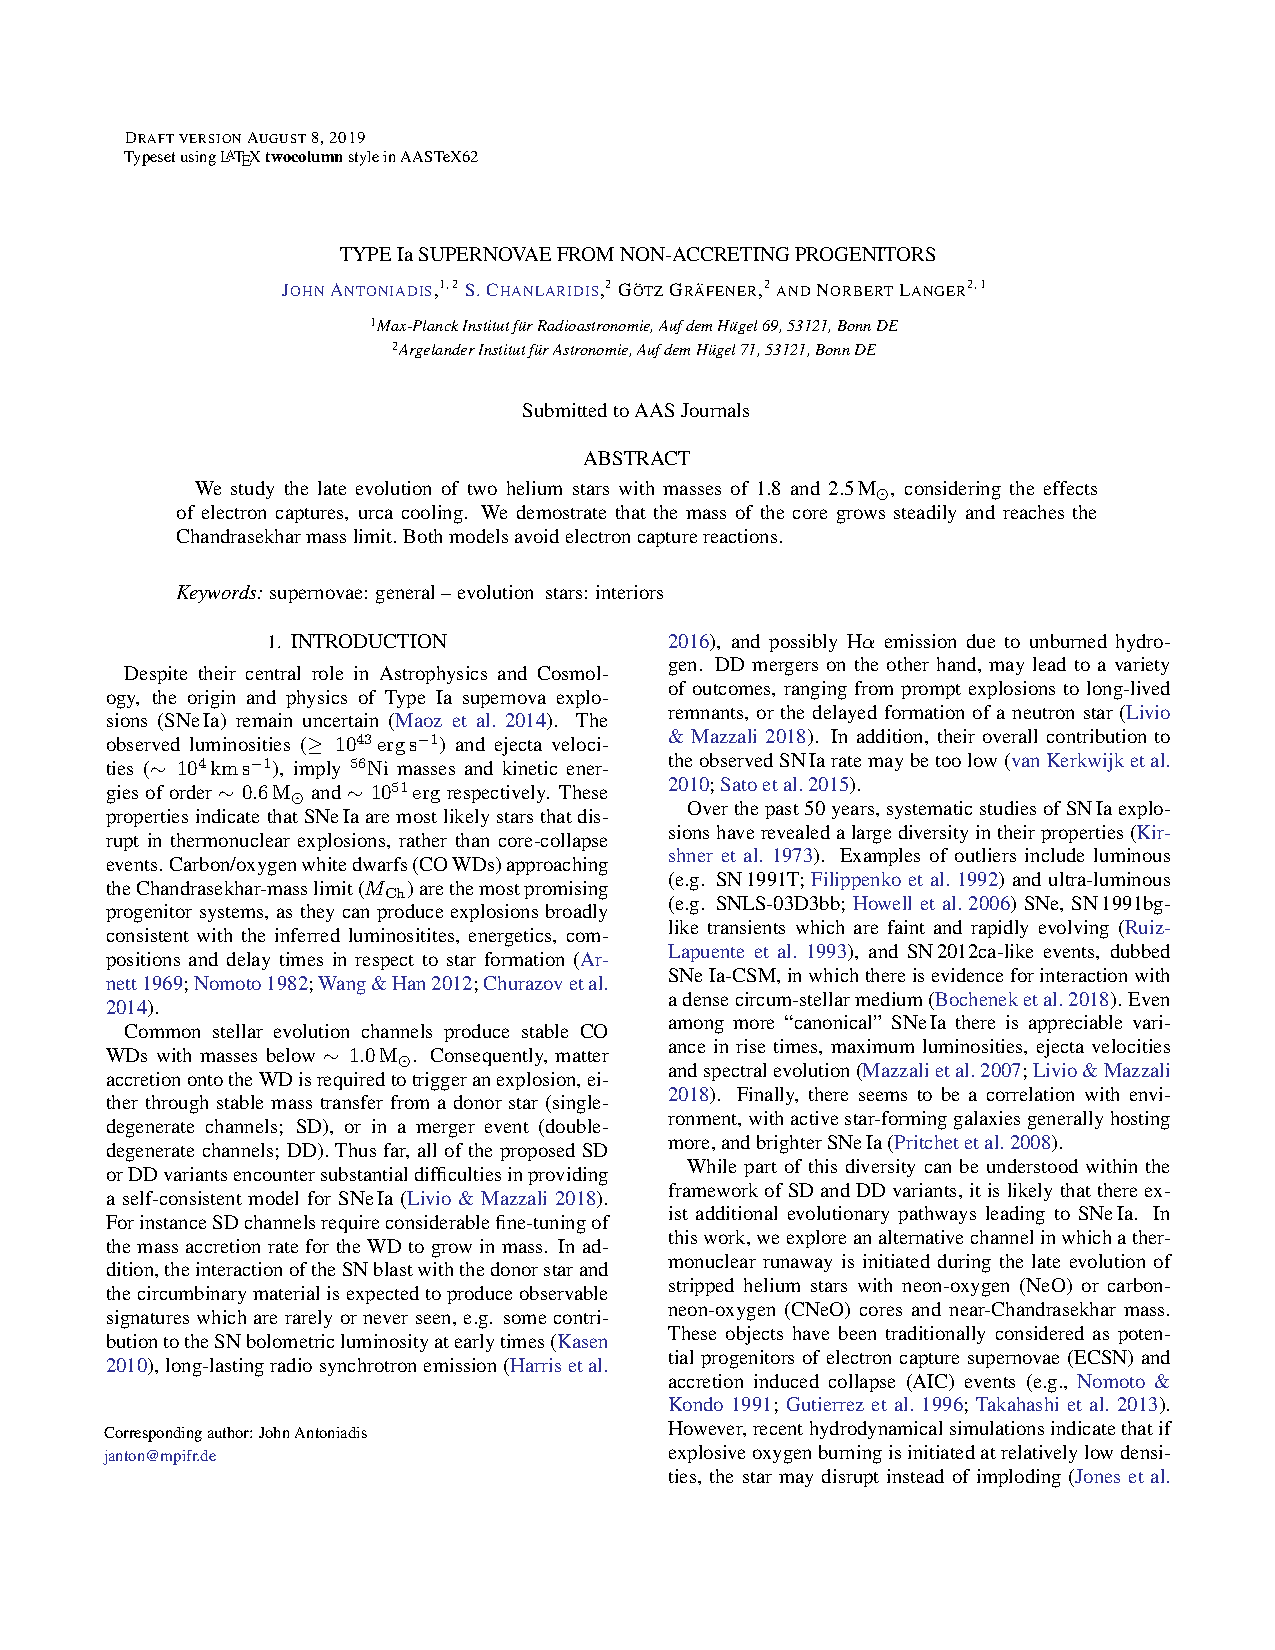
\includepdf[pages=-, scale=1.05, pagecommand={},frame=false, fitpaper=false,
            trim=0mm 0mm -10mm 0mm]{Supernovae.pdf}
            
           
            
            
     \null\newpage
     \section{Helium Stars as Progenitors of Thermonuclear Supernovae}\label{sec:results2}
     
     
    	 \vspace{3cm}
		
		In this section, we further explore the progenitor channel of SNe-Ia we described in section \ref{sec:results1}, by creating series of stellar models with various values of metallicity and overshoot mixing. We elaborate on the importance of residual carbon found in ONe cores, in initiating a thermal runaway leading to the disruption of the star.
		
		\vspace{15cm}
		\noindent \textbf{Disclaimer}: What follows is an early draft version of the manuscript submitted for publication to \textit{ApJ}. Differences may appear when compared with the published version. Hence, for citing this paper please refer to the journals.

\newpage

     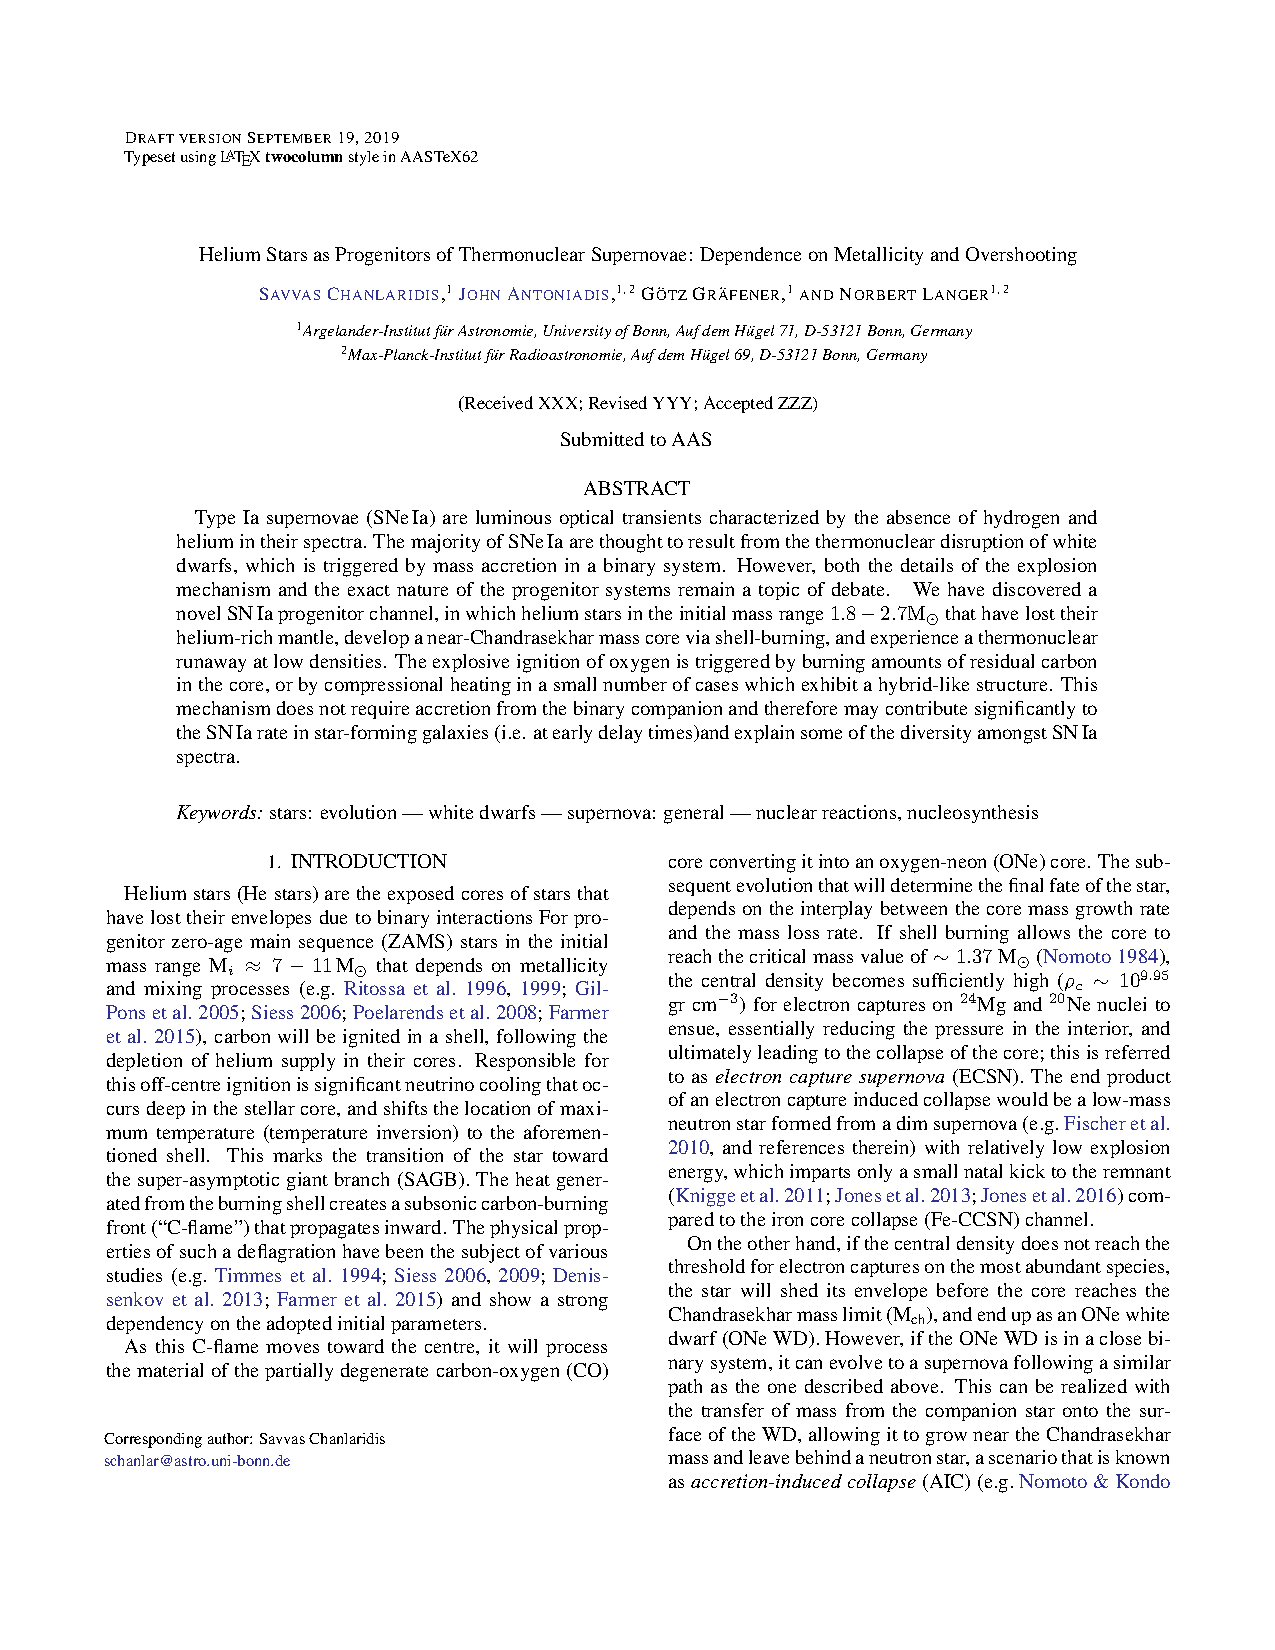
\includepdf[pages=-, scale=1.05, pagecommand={},frame=false, fitpaper=false,
            trim=0mm 0mm -10mm 0mm]{HeliumStars_SNeIa.pdf}
     
	

	
\end{document}